Analiza la figura geométrica obten la expresión algebraica para el \textbf{perímetro} de las siguientes figuras:

\begin{multicols}{2}
    \begin{parts}
        {\printanswers
        \part \centering 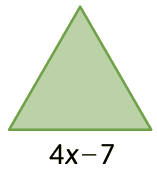
\includegraphics[width=0.12\textwidth]{../images/20230319042651}
        \begin{solutionbox}{3.5cm}\begin{align*}P=&(4x-7)+(4x-7)+(4x-7)\\=&4x-7+4x-7+4x-7\\=&4x+4x+4x-7-7-7\\=&12x-21\\    \end{align*}\end{solutionbox}
        }

        \part \centering 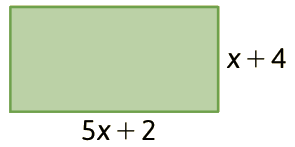
\includegraphics[width=0.24\textwidth]{../images/20230319042710}
        \begin{solutionbox}{3.5cm}\begin{align*}P=&(5x+2)+(x+4)+(5x+2)+(x+4)\\=&5x+2+x+4+5x+2+x+4\\=&5x +5x+x+x +4 +2 +4+2 \\=&12x+12 \end{align*}\end{solutionbox}

        \part \centering 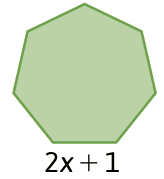
\includegraphics[width=0.12\textwidth]{../images/20230319042701}
        \begin{solutionbox}{3cm}\begin{align*}P=&7 \cdot (2x+1)\\=&14x+7     \end{align*}\end{solutionbox}

        \part \centering 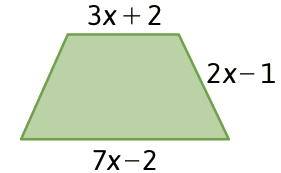
\includegraphics[width=0.22\textwidth]{../images/20230319042717}
        \begin{solutionbox}{3cm}\begin{align*}P=&(3x+2)+(2x-1)+(7x-2)+(2x-1)\\=&3x+2+2x-1+7x-2+2x-1\\=&14x-2\end{align*}\end{solutionbox}

    \end{parts}
\end{multicols}



